\section{Szymon Kozioł}

Wyrażenie matematyczne:
\[2+2*2 = 8^2 - 58\]

Zdjęcie:

\begin{figure}[h]
  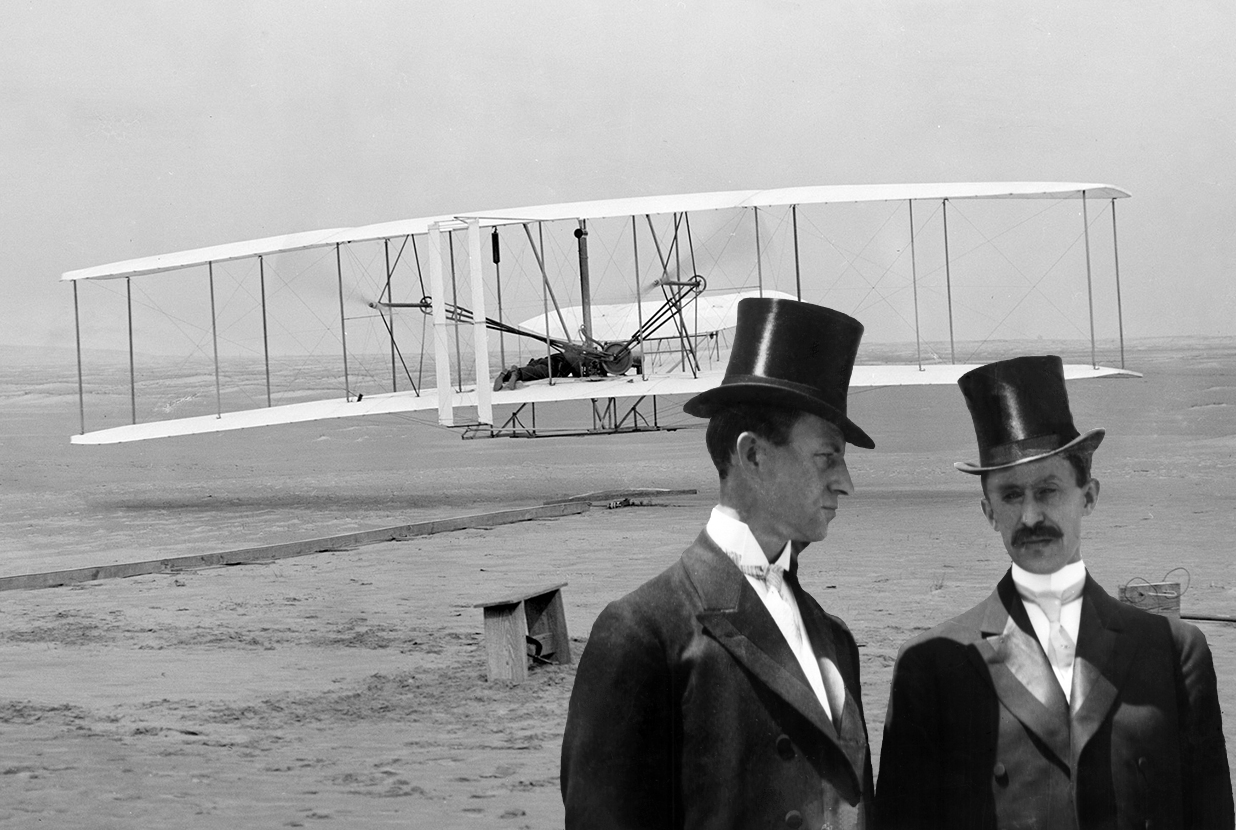
\includegraphics[width=11cm]{pictures/tacd}
  \centering
  \caption{Bracia Wright}
  \label{fig:bracia}
\end{figure}

Tabela:\newline
\begin{tabular}{lllll}
   &     k1)& k2) & k3) \\
rząd 1) & 1 & 7 & 5 &    \\
rząd 2) & 2 & 3 & 6 &    \\
\end{tabular}


Lista numerowana z Wikipedii:


\begin{enumerate}
  \item The first item
  \item The second item
  \item The third etc \ldots
\end{enumerate}

Lista nienumerowana:
\begin{itemize}
  \item[-->] raz
  \item[-->] dwa
  \item[<--] yzrt
\end{itemize}

\textbf{Niedźwiedź polarny} - gatunek dużego ssaka drapieżnego z rodziny niedźwiedziowatych, zamieszkującego Arktykę. Jest drapieżnikiem szczytowym w zasięgu swojego występowania. Grube futro i warstwa tłuszczu chronią go przed zimnem

\textbf{Bracia Wright}
\newline
Orville Wright (ur. 19 sierpnia 1871, zm. 30 stycznia 1948) i Wilbur Wright (ur. 16 kwietnia 1867, zm. 30 maja 1912) – amerykańscy pionierzy lotnictwa. Uważani są powszechnie za konstruktorów pierwszego udanego samolotu.
Rysunek:\ref{fig:bracia}
